\documentclass{article}
\usepackage{graphicx} % Required for inserting images
\usepackage{tikz} % Required for TikZ diagrams
\usetikzlibrary{positioning} % Required for positioning library
\usepackage{xcolor}
\usepackage{amssymb} % Required for checkmark symbol

\title{NexusForum - Cybersecurity}
\author{Iraklis Symeonidis}
\date{February 2026}

\begin{document}

\maketitle

\section{Introduction}

\section{NexusForum Security Framework}

This section presents the comprehensive security framework consisting of six layers integrated with five security verticals.

\subsection{Security Layers}

\begin{enumerate}
	\item \textbf{Orchestration} - Central coordination and management
	\item \textbf{User} - User identity and access management
	\item \textbf{Application/Service Centric Security} - Application and service-level security controls
	\item \textbf{Data Centric Security} - Data protection and privacy controls
	\item \textbf{Software/Middleware/OS Centric Security} - Operating system and middleware security
	\item \textbf{Device/Hardware Centric Security} - Physical device and hardware protection
\end{enumerate}

\subsection{Security Verticals}

\begin{enumerate}
	\item \textbf{Network} - Network infrastructure and perimeter security
	\item \textbf{Automation and Cyber-Resilient AI Lifecycle} - Automated security processes and AI integration
	\item \textbf{Dynamic Risk Management \& Operational Cyber Resilience} - Risk assessment and incident response
	\item \textbf{Interoperable Security Mechanisms} - Cross-platform security standards and integration
	\item \textbf{Agile Governance, Compliance-by-Design \& Automated Assurance} - Governance and compliance automation
\end{enumerate}

\subsection{Security Framework Matrix}

\begin{table}[h!]
	\centering
	\begin{tabular}{|l|c|c|c|c|c|}
		\hline
		\textbf{Layers / Verticals} & \textbf{Network} & \textbf{Automation \& AI} & \textbf{Risk Mgmt} & \textbf{Interoperable} & \textbf{Governance} \\
		\hline
		\textbf{Orchestration} & $\checkmark$ & $\checkmark$ & $\checkmark$ & $\checkmark$ & $\checkmark$ \\
		\hline
		\textbf{User} & $\checkmark$ & $\checkmark$ & $\checkmark$ & $\checkmark$ & $\checkmark$ \\
		\hline
		\textbf{Application/Service} & $\checkmark$ & $\checkmark$ & $\checkmark$ & $\checkmark$ & $\checkmark$ \\
		\hline
		\textbf{Data Centric} & $\checkmark$ & $\checkmark$ & $\checkmark$ & $\checkmark$ & $\checkmark$ \\
		\hline
		\textbf{Software/Middleware/OS} & $\checkmark$ & $\checkmark$ & $\checkmark$ & $\checkmark$ & $\checkmark$ \\
		\hline
		\textbf{Device/Hardware} & $\checkmark$ & $\checkmark$ & $\checkmark$ & $\checkmark$ & $\checkmark$ \\
		\hline
	\end{tabular}
	\caption{NexusForum Security Framework: Layers and Verticals Integration Matrix}
	\label{tab:security_framework}
\end{table}

\subsection{Security Framework Diagram}


	\begin{figure}[h!]
		\centering
		\resizebox{\textwidth}{!}{%
		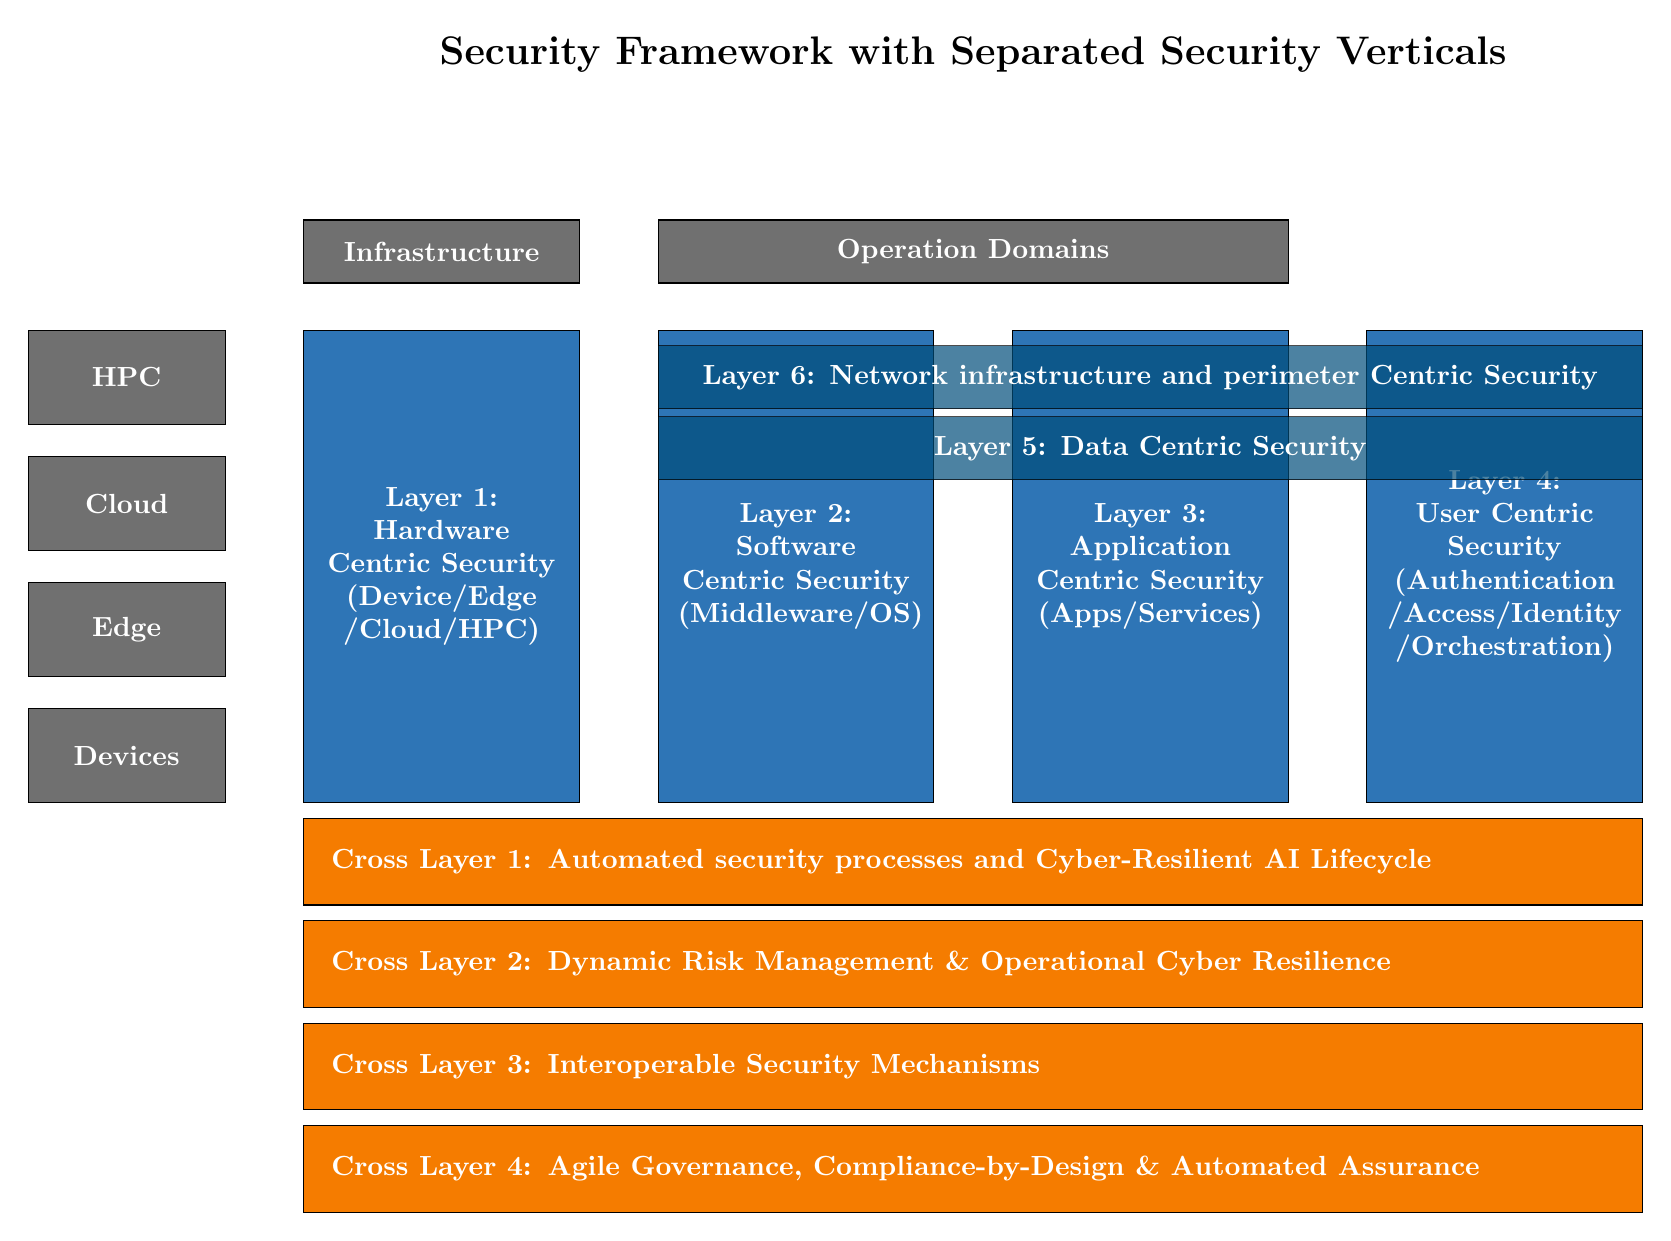
\begin{tikzpicture}[every node/.style={font=\small}]
			% Define colors
			\definecolor{archblue}{RGB}{46, 117, 182}
			\definecolor{sec_verticals_bg}{RGB}{245, 124, 0}
			\definecolor{env_bg}{RGB}{112, 112, 112}
			\definecolor{overlay}{RGB}{0, 77, 122}

			% Styles
			\tikzstyle{arch_col} = [fill=archblue, draw=black, text=white, font=\bfseries, minimum width=3.5cm, minimum height=6cm, align=center, text width=3cm]
			\tikzstyle{env_box} = [fill=env_bg, draw=black, text=white, font=\bfseries, minimum width=2.5cm, minimum height=1.2cm, align=center]
			\tikzstyle{top_tool} = [draw=black, fill=env_bg, text=white, minimum height=0.8cm, align=center, font=\bfseries]
			\tikzstyle{overlay_box} = [fill=overlay, draw=black, text=white, font=\bfseries, minimum height=0.8cm, align=center, opacity=0.7, text opacity=1]
			\tikzstyle{vertical_box} = [fill=sec_verticals_bg, draw=black, text=white, font=\bfseries, minimum width=17.0cm, minimum height=1.1cm, align=left, text width=16.3cm]

			% Column X positions
			\def\colone{-4.5}
			\def\coltwo{0}
			\def\colthree{4.5}
			\def\colfour{9}

			% Environment boxes (left)
			\node[env_box] at (-8.5, 2.4) {HPC};
			\node[env_box] at (-8.5, 0.8) {Cloud};
			\node[env_box] at (-8.5, -0.8) {Edge};
			\node[env_box] at (-8.5, -2.4) {Devices};

			% Main architecture columns representing layers
			\node[arch_col] (hw) at (\colone, 0) {Layer 1: \\ Hardware Centric Security \\ (Device/Edge\\ /Cloud/HPC)};
			\node[arch_col] (mw) at (\coltwo, 0) {Layer 2: \\ Software Centric Security \\ (Middleware/OS)};
			\node[arch_col] (app) at (\colthree, 0) {Layer 3: \\ Application Centric Security \\ (Apps/Services)};
			\node[arch_col] (user) at (\colfour, 0) {Layer 4: \\ User Centric Security \\ (Authentication\\ /Access/Identity\\ /Orchestration)};

			% Top tooling boxes
			\node[top_tool, minimum width=3.5cm] at (\colone, 4) {Infrastructure};
			\node[top_tool, minimum width=8cm] at (2.25, 4) {Operation Domains};

			% Arrows from tooling
			\draw[->, line width=2pt, white] (\colone, 3.5) -- (\colone, 3.1);
			\draw[->, line width=2pt, white] (2.25, 3.5) -- (2.25, 3.1);

			% Other layers as overlays/headers
			\node[overlay_box, minimum width=12.5cm] at (4.5, 1.5) {Layer 5: Data Centric Security};
			\node[overlay_box, minimum width=12.5cm] at (4.5, 2.4) {Layer 6: Network infrastructure and perimeter Centric Security};

			% Separated vertical boxes
			\node[vertical_box] at (2.25, -3.75) {\textbf{Cross Layer 1: Automated security processes and Cyber-Resilient AI Lifecycle}};
			\node[vertical_box] at (2.25, -5.05) {\textbf{Cross Layer 2: Dynamic Risk Management \& Operational Cyber Resilience}};
			\node[vertical_box] at (2.25, -6.35) {\textbf{Cross Layer 3: Interoperable Security Mechanisms}};
			\node[vertical_box] at (2.25, -7.65) {\textbf{Cross Layer 4: Agile Governance, Compliance-by-Design \& Automated Assurance}};

			% Title
			\node[font=\Large\bfseries, anchor=center] at (2.25, 6.5) {Security Framework with Separated Security Verticals};

		\end{tikzpicture}%
		}
		\caption{Security Framework with separated security verticals in dedicated boxes.}
		\label{fig:security_framework_verticals_boxes}
	\end{figure}
	

\begin{figure}[h!]
	\centering
	\resizebox{\textwidth}{!}{%
	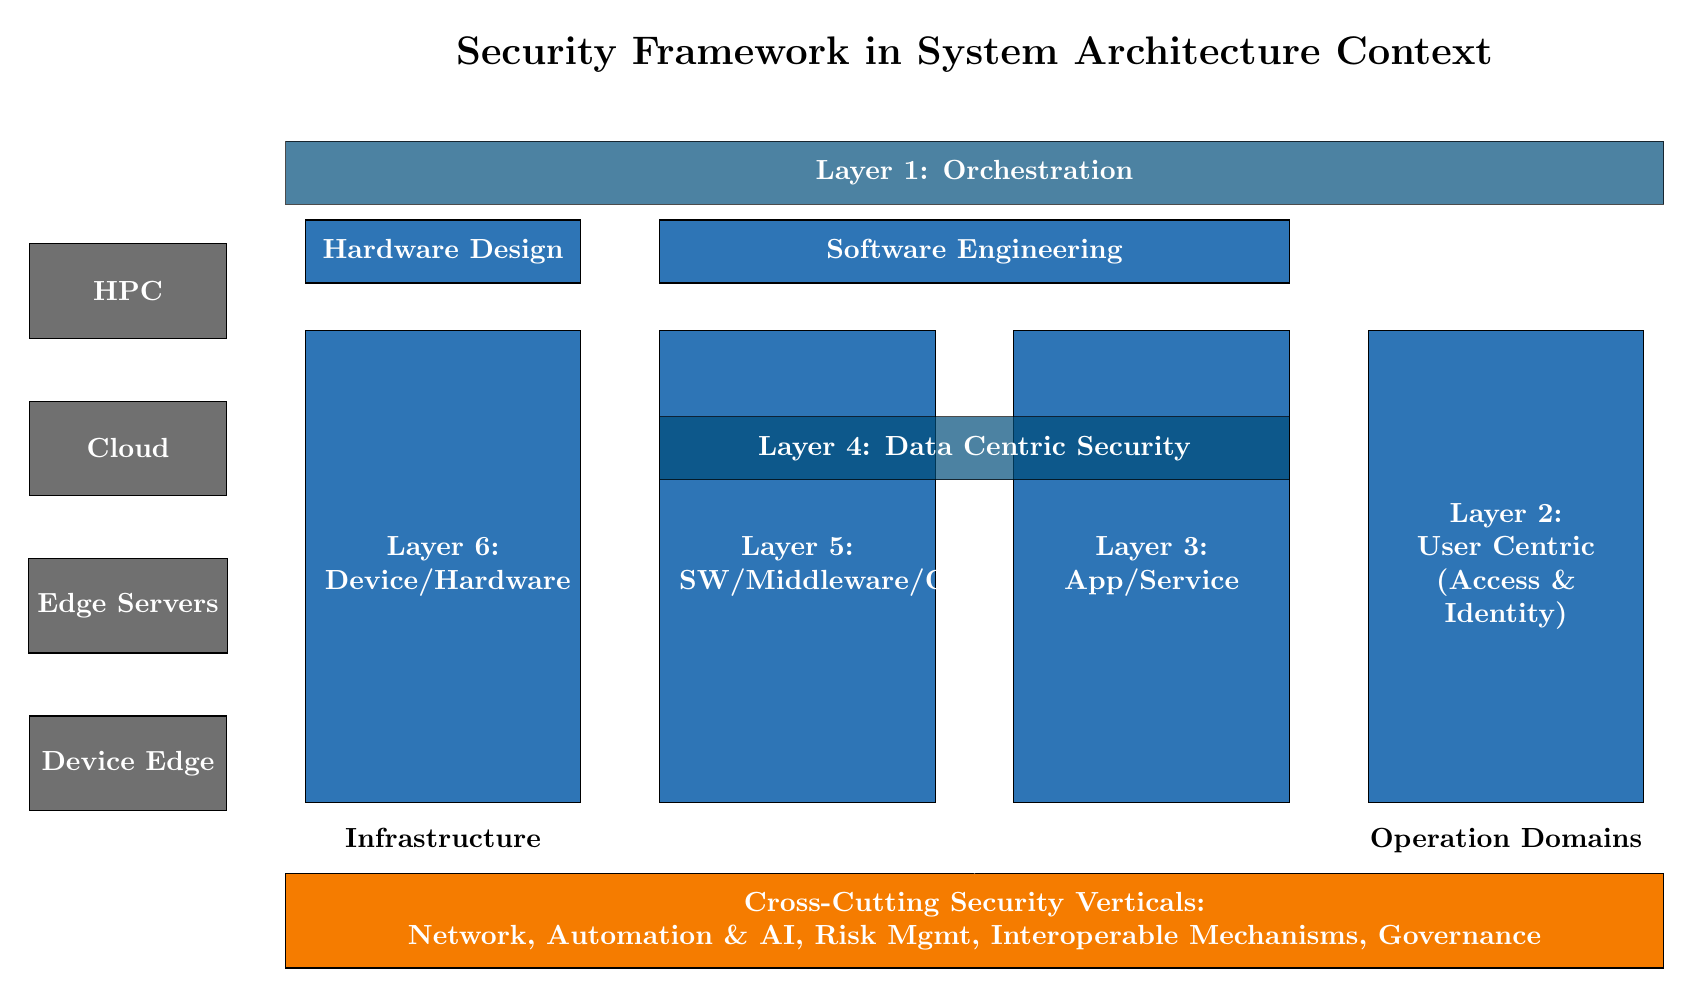
\begin{tikzpicture}[every node/.style={font=\small}]
		% Define colors
		\definecolor{archblue}{RGB}{46, 117, 182} % Similar to reference PDF
		\definecolor{sec_verticals_bg}{RGB}{245, 124, 0} % Orange for verticals bar
		\definecolor{env_bg}{RGB}{112, 112, 112}
		\definecolor{overlay}{RGB}{0, 77, 122}

		% Styles
		\tikzstyle{arch_col} = [fill=archblue, draw=black, text=white, font=\bfseries, minimum width=3.5cm, minimum height=6cm, align=center, text width=3cm]
		\tikzstyle{env_box} = [fill=env_bg, draw=black, text=white, font=\bfseries, minimum width=2.5cm, minimum height=1.2cm, align=center]
		\tikzstyle{bottom_bar} = [fill=sec_verticals_bg, draw=black, text=white, font=\bfseries, minimum width=11.5cm, minimum height=1.2cm, align=center, text width=11cm]
		\tikzstyle{top_tool} = [draw=black, fill=archblue, text=white, minimum height=0.8cm, align=center, font=\bfseries]
		\tikzstyle{layer_label} = [font=\bfseries\large, align=center]
		\tikzstyle{overlay_box} = [fill=overlay, draw=black, text=white, font=\bfseries, minimum height=0.8cm, align=center, opacity=0.7, text opacity=1]

		% Column X positions
		\def\colone{-4.5}
		\def\coltwo{0}
		\def\colthree{4.5}
		\def\colfour{9}

		% Environment boxes (left)
		\node[env_box] at (-8.5, 3.5) {HPC};
		\node[env_box] at (-8.5, 1.5) {Cloud};
		\node[env_box] at (-8.5, -0.5) {Edge Servers};
		\node[env_box] at (-8.5, -2.5) {Device Edge};

		% Main architecture columns representing layers
		\node[arch_col] (hw) at (\colone, 0) {Layer 6: \\ Device/Hardware};
		\node[arch_col] (mw) at (\coltwo, 0) {Layer 5: \\ SW/Middleware/OS};
		\node[arch_col] (app) at (\colthree, 0) {Layer 3: \\ App/Service};
		\node[arch_col] (user) at (\colfour, 0) {Layer 2: \\ User Centric (Access \& Identity)};

		% Labels for columns
		\node[below=0.2cm of hw, font=\bfseries, anchor=north] {Infrastructure};
		\node[below=0.2cm of user, font=\bfseries, anchor=north] {Operation Domains};

		% Top tooling boxes
		\node[top_tool, minimum width=3.5cm] at (\colone, 4) {Hardware Design};
		\node[top_tool, minimum width=8cm] at (2.25, 4) {Software Engineering};
		
		% Arrows from tooling
		\draw[->, line width=2pt, white] (\colone, 3.5) -- (\colone, 3.1);
		\draw[->, line width=2pt, white] (2.25, 3.5) -- (2.25, 3.1);

		% Other layers as overlays/headers
		\node[overlay_box, minimum width=8cm] at (2.25, 1.5) {Layer 4: Data Centric Security};
		\node[overlay_box, minimum width=17.5cm] at (2.25, 5) {Layer 1: Orchestration};

		% Bottom bar for Security Verticals
		\node[bottom_bar, minimum width=17.5cm, text width=17cm] at (2.25, -4.5) {Cross-Cutting Security Verticals: \\ Network, Automation \& AI, Risk Mgmt, Interoperable Mechanisms, Governance};
		
		% Arrow to bottom bar
		\draw[<->, line width=2pt, white] (2.25, -3.5) -- (2.25, -3.9);

		% Title
		\node[font=\Large\bfseries, anchor=center] at (2.25, 6.5) {Security Framework in System Architecture Context};

	\end{tikzpicture}%
	}
	\caption{Security Framework in a System Architecture Context, inspired by the reference draft.}
	\label{fig:security_framework}
\end{figure}



\subsection{Layered Stack with Vertical Spans}

\begin{figure}[h!]
	\centering
	\resizebox{\textwidth}{!}{%
	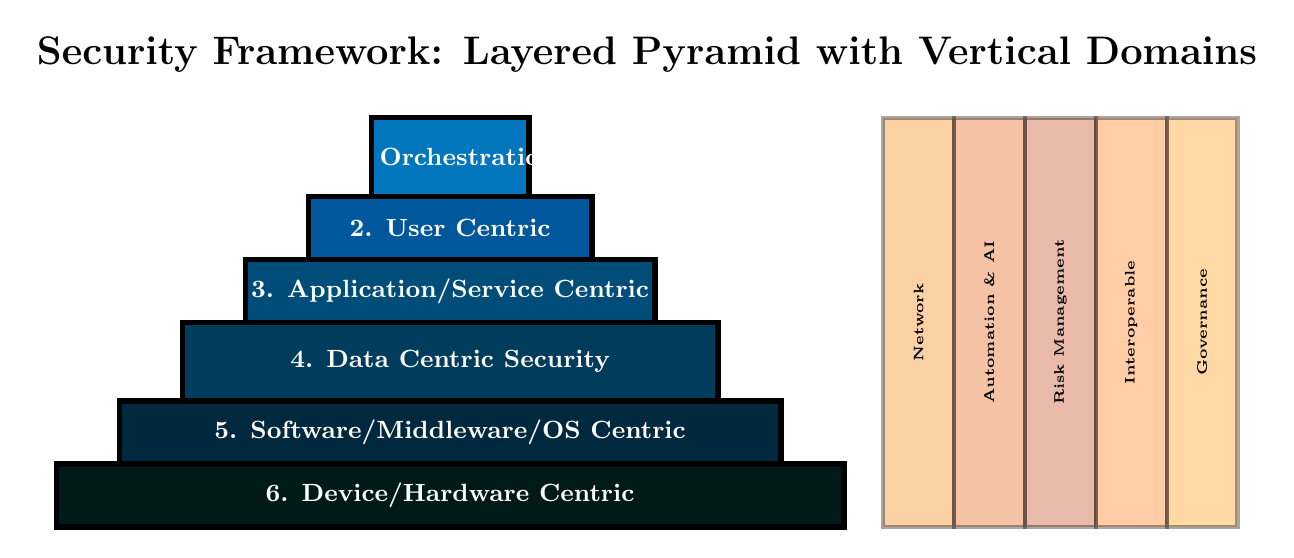
\begin{tikzpicture}[every node/.style={font=\small}]
		% Define colors
		\definecolor{layer1}{RGB}{2, 119, 189}
		\definecolor{layer2}{RGB}{1, 87, 155}
		\definecolor{layer3}{RGB}{0, 77, 122}
		\definecolor{layer4}{RGB}{0, 61, 92}
		\definecolor{layer5}{RGB}{0, 41, 64}
		\definecolor{layer6}{RGB}{0, 26, 26}
		\definecolor{vert1}{RGB}{245, 124, 0}
		\definecolor{vert2}{RGB}{230, 81, 0}
		\definecolor{vert3}{RGB}{191, 54, 12}
		\definecolor{vert4}{RGB}{255, 111, 0}
		\definecolor{vert5}{RGB}{255, 143, 0}
		
		% ===== PYRAMID LAYERS (Bottom to Top) =====
		% Layer 6 - Device/Hardware (widest, bottom)
		\draw[fill=layer6, draw=black, line width=2pt] (0, 0) -- (10, 0) -- (10, 0.8) -- (0, 0.8) -- cycle;
		\node[text=white, font=\small\bfseries, anchor=center] at (5, 0.4) {6. Device/Hardware Centric};
		
		% Layer 5
		\draw[fill=layer5, draw=black, line width=2pt] (0.8, 0.8) -- (9.2, 0.8) -- (9.2, 1.6) -- (0.8, 1.6) -- cycle;
		\node[text=white, font=\small\bfseries, anchor=center] at (5, 1.2) {5. Software/Middleware/OS Centric};
		
		% Layer 4
		\draw[fill=layer4, draw=black, line width=2pt] (1.6, 1.6) -- (8.4, 1.6) -- (8.4, 2.6) -- (1.6, 2.6) -- cycle;
		\node[text=white, font=\small\bfseries, anchor=center] at (5, 2.1) {4. Data Centric Security};
		
		% Layer 3
		\draw[fill=layer3, draw=black, line width=2pt] (2.4, 2.6) -- (7.6, 2.6) -- (7.6, 3.4) -- (2.4, 3.4) -- cycle;
		\node[text=white, font=\small\bfseries, anchor=center] at (5, 3.0) {3. Application/Service Centric};
		
		% Layer 2
		\draw[fill=layer2, draw=black, line width=2pt] (3.2, 3.4) -- (6.8, 3.4) -- (6.8, 4.2) -- (3.2, 4.2) -- cycle;
		\node[text=white, font=\small\bfseries, anchor=center] at (5, 3.8) {2. User Centric};
		
		% Layer 1 - Orchestration (narrowest, top)
		\draw[fill=layer1, draw=black, line width=2pt] (4, 4.2) -- (6, 4.2) -- (6, 5.2) -- (4, 5.2) -- cycle;
		\node[text=white, font=\small\bfseries, anchor=center] at (5, 4.7) {1. Orchestration};
		
		% ===== VERTICAL SPANS (Semi-transparent overlays) =====
		% Vertical 1 - Network
		\draw[fill=vert1, draw=black, line width=1.5pt, opacity=0.35] (10.5, 0) -- (11.4, 0) -- (11.4, 5.2) -- (10.5, 5.2) -- cycle;
		\node[text=black, font=\tiny\bfseries, anchor=center, rotate=90] at (10.95, 2.6) {Network};
		
		% Vertical 2
		\draw[fill=vert2, draw=black, line width=1.5pt, opacity=0.35] (11.4, 0) -- (12.3, 0) -- (12.3, 5.2) -- (11.4, 5.2) -- cycle;
		\node[text=black, font=\tiny\bfseries, anchor=center, rotate=90] at (11.85, 2.6) {Automation \& AI};
		
		% Vertical 3
		\draw[fill=vert3, draw=black, line width=1.5pt, opacity=0.35] (12.3, 0) -- (13.2, 0) -- (13.2, 5.2) -- (12.3, 5.2) -- cycle;
		\node[text=black, font=\tiny\bfseries, anchor=center, rotate=90] at (12.75, 2.6) {Risk Management};
		
		% Vertical 4
		\draw[fill=vert4, draw=black, line width=1.5pt, opacity=0.35] (13.2, 0) -- (14.1, 0) -- (14.1, 5.2) -- (13.2, 5.2) -- cycle;
		\node[text=black, font=\tiny\bfseries, anchor=center, rotate=90] at (13.65, 2.6) {Interoperable};
		
		% Vertical 5
		\draw[fill=vert5, draw=black, line width=1.5pt, opacity=0.35] (14.1, 0) -- (15, 0) -- (15, 5.2) -- (14.1, 5.2) -- cycle;
		\node[text=black, font=\tiny\bfseries, anchor=center, rotate=90] at (14.55, 2.6) {Governance};
		
		% Title
		\node[font=\Large\bfseries, anchor=center] at (7.5, 6.0) {Security Framework: Layered Pyramid with Vertical Domains};
		
	\end{tikzpicture}%
	}
	\caption{Security Layers as Pyramid Stack with Vertical Security Domains Spanning All Layers}
	\label{fig:pyramid_with_verticals}
\end{figure}

\subsection{Integrated Layers and Verticals Overview}

\begin{figure}[h!]
	\centering
	\resizebox{\textwidth}{!}{%
	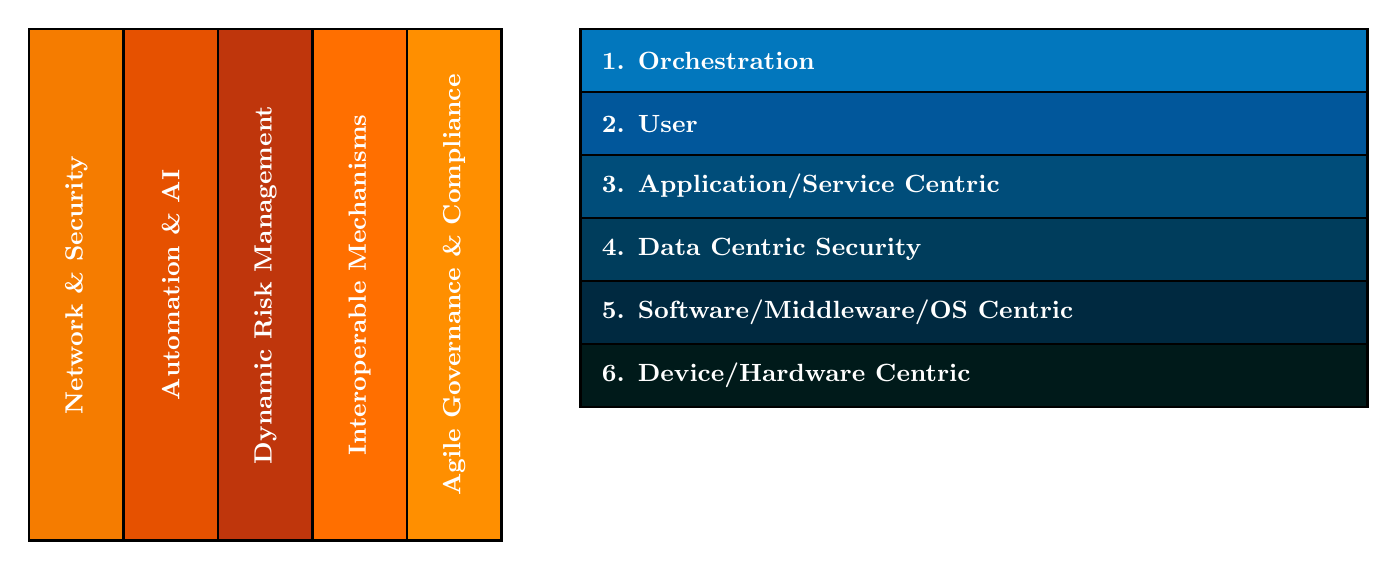
\begin{tikzpicture}[every node/.style={font=\small}]
		% Define colors
		\definecolor{layer1}{RGB}{2, 119, 189}
		\definecolor{layer2}{RGB}{1, 87, 155}
		\definecolor{layer3}{RGB}{0, 77, 122}
		\definecolor{layer4}{RGB}{0, 61, 92}
		\definecolor{layer5}{RGB}{0, 41, 64}
		\definecolor{layer6}{RGB}{0, 26, 26}
		\definecolor{vert1}{RGB}{245, 124, 0}
		\definecolor{vert2}{RGB}{230, 81, 0}
		\definecolor{vert3}{RGB}{191, 54, 12}
		\definecolor{vert4}{RGB}{255, 111, 0}
		\definecolor{vert5}{RGB}{255, 143, 0}
		
		% LEFT SIDE: VERTICALS (Colored Bars)
		% Vertical 1 - Network & Security
		\draw[fill=vert1, draw=black, line width=1pt] (0, 0) -- (1.2, 0) -- (1.2, 6.5) -- (0, 6.5) -- cycle;
		\node[text=white, font=\small\bfseries, anchor=center, rotate=90] at (0.6, 3.25) {Network \& Security};
		
		% Vertical 2 - Automation & AI
		\draw[fill=vert2, draw=black, line width=1pt] (1.2, 0) -- (2.4, 0) -- (2.4, 6.5) -- (1.2, 6.5) -- cycle;
		\node[text=white, font=\small\bfseries, anchor=center, rotate=90] at (1.8, 3.25) {Automation \& AI};
		
		% Vertical 3 - Dynamic Risk Management
		\draw[fill=vert3, draw=black, line width=1pt] (2.4, 0) -- (3.6, 0) -- (3.6, 6.5) -- (2.4, 6.5) -- cycle;
		\node[text=white, font=\small\bfseries, anchor=center, rotate=90] at (3.0, 3.25) {Dynamic Risk Management};
		
		% Vertical 4 - Interoperable
		\draw[fill=vert4, draw=black, line width=1pt] (3.6, 0) -- (4.8, 0) -- (4.8, 6.5) -- (3.6, 6.5) -- cycle;
		\node[text=white, font=\small\bfseries, anchor=center, rotate=90] at (4.2, 3.25) {Interoperable Mechanisms};
		
		% Vertical 5 - Governance
		\draw[fill=vert5, draw=black, line width=1pt] (4.8, 0) -- (6.0, 0) -- (6.0, 6.5) -- (4.8, 6.5) -- cycle;
		\node[text=white, font=\small\bfseries, anchor=center, rotate=90] at (5.4, 3.25) {Agile Governance \& Compliance};
		
		% RIGHT SIDE: LAYERS (Horizontal Bars)
		% Gap between left and right
		\def\rightstart{7.0}
		\def\barwidth{10}
		
		% Layer 1 - Orchestration
		\draw[fill=layer1, draw=black, line width=1pt] (\rightstart, 5.7) -- (\rightstart+\barwidth, 5.7) -- (\rightstart+\barwidth, 6.5) -- (\rightstart, 6.5) -- cycle;
		\node[text=white, font=\small\bfseries, anchor=west] at (\rightstart+0.15, 6.1) {1. Orchestration};
		
		% Layer 2 - User
		\draw[fill=layer2, draw=black, line width=1pt] (\rightstart, 4.9) -- (\rightstart+\barwidth, 4.9) -- (\rightstart+\barwidth, 5.7) -- (\rightstart, 5.7) -- cycle;
		\node[text=white, font=\small\bfseries, anchor=west] at (\rightstart+0.15, 5.3) {2. User};
		
		% Layer 3 - Application/Service
		\draw[fill=layer3, draw=black, line width=1pt] (\rightstart, 4.1) -- (\rightstart+\barwidth, 4.1) -- (\rightstart+\barwidth, 4.9) -- (\rightstart, 4.9) -- cycle;
		\node[text=white, font=\small\bfseries, anchor=west] at (\rightstart+0.15, 4.5) {3. Application/Service Centric};
		
		% Layer 4 - Data Centric
		\draw[fill=layer4, draw=black, line width=1pt] (\rightstart, 3.3) -- (\rightstart+\barwidth, 3.3) -- (\rightstart+\barwidth, 4.1) -- (\rightstart, 4.1) -- cycle;
		\node[text=white, font=\small\bfseries, anchor=west] at (\rightstart+0.15, 3.7) {4. Data Centric Security};
		
		% Layer 5 - Software/Middleware/OS
		\draw[fill=layer5, draw=black, line width=1pt] (\rightstart, 2.5) -- (\rightstart+\barwidth, 2.5) -- (\rightstart+\barwidth, 3.3) -- (\rightstart, 3.3) -- cycle;
		\node[text=white, font=\small\bfseries, anchor=west] at (\rightstart+0.15, 2.9) {5. Software/Middleware/OS Centric};
		
		% Layer 6 - Device/Hardware
		\draw[fill=layer6, draw=black, line width=1pt] (\rightstart, 1.7) -- (\rightstart+\barwidth, 1.7) -- (\rightstart+\barwidth, 2.5) -- (\rightstart, 2.5) -- cycle;
		\node[text=white, font=\small\bfseries, anchor=west] at (\rightstart+0.15, 2.1) {6. Device/Hardware Centric};
		
	\end{tikzpicture}
	}
	\caption{NexusForum Security Framework: Layers and Verticals Integration}
	\label{fig:layers_verticals_overview}
\end{figure}

\end{document}
